\documentclass[a4paper]{article}

%%%%%%%%%%%%%%%%%%%%%%%%%%%%%%%%%%%%%%%%%%%%%%
\usepackage[T1]{fontenc}
\usepackage{geometry}
\geometry{a4paper,left=1.5cm,right=1cm,top=1cm,bottom=1cm}

\usepackage{graphicx}
\usepackage[absolute,overlay]{textpos}
\usepackage{eso-pic}               % image de fond
\usepackage{fontawesome5}
\usepackage[hidelinks]{hyperref}
\usepackage{tikz}
\usepackage{xcolor}
\usepackage{enumitem}
\setlist{nosep,leftmargin=6mm}
\usepackage{times}                % même police que votre exemple
\usepackage{array} 
\usepackage{tabularx}
\usepackage{ragged2e}

\let\origcolorbox\colorbox    % sauvegarde
\renewcommand{\colorbox}[2]{#2}% neutralise le fond
%%%%%%%%%%%%%%%%%%%%%%%%%%%%%%%%%%%%%%%%%%%%%%
%\definecolor{texcolor}{HTML}{e2e8f0}
\providecolor{sidetext}{rgb}{1,1,1}
\definecolor{maincolor}{HTML}{ffffff}

%%%%%%%%%%%%%%%%%%%%%%%%%%%%%%%%%%%%%%%%%
% — Ne changez pas le nom : « background.jpg » doit être présent
\AddToShipoutPictureBG*{%
  
\includegraphics[width=\paperwidth,height=\paperheight]{background.jpg}%
}

%%%%%%%%%%%%%%%%%%%%%%%%%%%%%%%%%%%%%%%%%
\newcommand{\fullrule}{\hspace{-1.5cm}\rule{\paperwidth}{0.4pt}}
\newcommand{\cvsection}[1]{%
  \vspace{6pt}\textbf{\Large #1}\par\vspace{2pt}}
\newcommand{\cicon}[1]{%
  \tikz[baseline]{\draw[fill=white] (0,0.1) circle[radius=0.1cm];}~#1}

\setlength{\parindent}{0pt}
%\color{texcolor}
%%%%%%%%%%%%%%%%%%%%%%%%%%%%%%%%%%%%%%%%%%%%%%%%%%%%%%%%%%%%%%
\begin{document}
\color{white}
% ---------- Photo ------------------------------------------------
\begin{textblock*}{4cm}(0.2cm,0.3cm)
  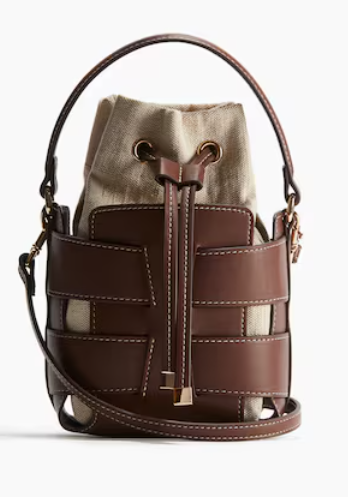
\includegraphics[width=2.5cm,clip,keepaspectratio]{ba7717b66a454673a00074fee5d8041c.png}
\end{textblock*}

% ---------- En-tête ---------------------------------------------
\begin{center}
  {\fontsize{44pt}{24pt}\selectfont\bfseries Judikael Mourouvin}

  \bigskip
  {\Large Technicien Informatique \& Marketing Digital}

  \bigskip\bigskip
  \faMapMarker~Route de Cocoyer\ 97190 Gosier
  \quad\faEnvelope~\href{mailto:jkmou971@gmail.com}{jkmou971@gmail.com}

  \bigskip
  % Badge LinkedIn (retirez-le si inutile)
  \faPhone~ +590 0690 91 14 48
  \quad \faLinkedin\ \href{}{}
 

  \vspace{-0.3cm}
  \fullrule
\end{center}

% ---------- Profil ----------------------------------------------
\cvsection{Profil}
\hspace*{2.2cm}%
Passionné par l’informatique et le marketing digital, j’ai développé une double compétence en support technique et en communication en ligne. Mon année d’alternance à la DSI de la Mairie du Gosier m’a permis de gérer des projets numériques tout en formant les utilisateurs. J’apprécie particulièrement d’analyser les besoins pour proposer des solutions fiables et efficaces. Désormais, je souhaite m’investir à plein temps afin de contribuer à vos projets avec rigueur et réactivité.

\medskip\fullrule

% ---------- Expérience ------------------------------------------
\cvsection{Expérience}
\hspace*{1.3cm}%

\colorbox{maincolor}{%
  \begin{minipage}{\linewidth}
    \textbf{Alternant en Marketing Digital} \\ Mairie du Gosier - DSI \\ 2023-2024
    \begin{itemize}
      \item Piloté divers projets numériques, renforçant la visibilité en ligne de la collectivité. \item Analysé les besoins des usagers et déployé des solutions adaptées, réduisant les délais de traitement. \item Assuré support et formation aux utilisateurs, favorisant l’adoption des outils digitaux.
    \end{itemize}
  \end{minipage}}

\vspace{3mm}


\colorbox{maincolor}{%
  \begin{minipage}{\linewidth}
    \textbf{Animateur de la zone informatique} \\ Pôle Emploi, Gosier \\ 2022-2023
    \begin{itemize}
      \item Guidé quotidiennement les utilisateurs sur les postes en libre accès, améliorant leur autonomie. \item Configuré et entretenu le parc informatique, diminuant les pannes matérielles. \item Diagnostiqué et résolu les incidents, réduisant le temps d’indisponibilité des équipements.
    \end{itemize}
  \end{minipage}}

\vspace{3mm}


\colorbox{maincolor}{%
  \begin{minipage}{\linewidth}
    \textbf{Stagiaire Informaticien} \\ Numerika, Baie-Mahault \\ 2020-2021
    \begin{itemize}
      \item Installé et maintenu postes et périphériques, optimisant la performance du parc. \item Fournit un support technique de premier niveau, améliorant la satisfaction des utilisateurs.
    \end{itemize}
  \end{minipage}}

\medskip\fullrule

% ---------- Éducation -------------------------------------------
\cvsection{Éducation}
\hspace*{1.3cm}%

    \begin{tabularx}{\linewidth}{@{}c >{\RaggedRight\arraybackslash}X@{}}
    \textcolor{sidetext}{\faGraduationCap} &
    \textbf{Bachelor Marketing Digital} \\
    & CFA IUTS \\
    & \textit{2023-2024} \\
    \end{tabularx}
    \begin{itemize}[leftmargin=*]
  \item Stratégies de communication numérique et gestion de campagnes en ligne.
  \item Analyse de données marketing et optimisation du parcours client.
  \item Maîtrise des outils SEO, SEA et des réseaux sociaux pour accroître la visibilité.
\end{itemize}
\vspace{3mm}

    \begin{tabularx}{\linewidth}{@{}c >{\RaggedRight\arraybackslash}X@{}}
    \textcolor{sidetext}{\faGraduationCap} &
    \textbf{BTS Systèmes Numériques option Informatique et Réseaux} \\
    & Lycée de Chevalier Saint Georges, Abymes \\
    & \textit{2019-2021} \\
    \end{tabularx}
    \begin{itemize}[leftmargin=*]
  \item Administration de réseaux locaux et configuration d’équipements.
  \item Dépannage matériel/logiciel et gestion de parc informatique.
  \item Conception et maintenance de systèmes connectés et applications embarquées.
\end{itemize}

\medskip\fullrule

% ---------- Compétences -----------------------------------------
\cvsection{Compétences}
\\
\hspace*{2.2cm}%
\begin{tabular}{@{}p{0.25\linewidth}p{0.18\linewidth}p{0.18\linewidth}p{0.18\linewidth}}\cicon Administration & \cicon Réseaux & \cicon Support & \cicon Maintenance \\
\cicon Marketing & \cicon Digital & \cicon Assistance & \cicon Configuration \\
\cicon Diagnostic & \cicon Gestion & ~ & ~ \\\end{tabular}   % grille 3 lignes × 4 colonnes

\end{document}
